%!TEX root = mieic.tex
\chapter{Metodologia} \label{chap:metod}

\section*{}

Neste capítulo é descrita de uma forma sucinta a metodologia usada para alcançar os objetivos propostos. São definidos alguns conceitos importantes para o correto desenvolvimento, bem como as diferentes etapas inicialmente definidas que permitirão atingir o desejado.

\section{Definições e Terminologia}

Neste projeto, de acordo com o que é pretendido, é possível distinguir dois utilizadores finais, o programador que usará a \textit{framework} desenvolvida e o transeunte que utilizará a aplicação do ecrã público. Tendo em conta este último, será adequado considerar dois conceitos relacionados, sendo eles Interação Pessoa-Computador(IPC) e Desenvolvimento Centrado no Utilizador(DCU).

IPC é uma área focada no \textit{design}, avaliação e implementação de sistemas interativos para uso antrópico, dando relevância à satisfação do utilizador final. 
Enquanto a engenharia de \textit{software} se preocupa com a produção de soluções para aplicações de \textit{software}, IPC foca-se em descobrir métodos e técnicas que melhorem a interação entre pessoa-computador.


Existem algumas razões que fazem com que IPC seja uma área de estudo com valor, muito ativa e em franca expansão~\cite{smith2006human}:
\begin{itemize}
	\item Considera como principal no desenvolvimento de aplicações o utilizador final e preocupa-se com ele durante todas as fases de desenvolvimento.
	\item Fornece uma base sobre a qual é possível avaliar métodos de \textit{design} para a sua eficiência e eficácia. O desenvolvimento de um sistema necessita de várias formas para avaliar os métodos usados, que podem ser obtidos através de IPC.
	\item Proporciona um ambiente baseado no mundo real, permitindo novas teorias baseadas na psicologia humana. E este campo é uma das áreas de crescimento mais rápido no campo da ciência da computação.
\end{itemize}

\subsection*{Desenvolvimento Centrado no Utilizador}

DCU é um conceito para descrever os projetos nos quais o foco central é o utilizador final. É ao mesmo tempo uma filosofia ampla com vários métodos, pois há diversas maneiras através das quais os utilizadores são envolvidos. Uma metodologia baseada em DCU interessa-se pelas necessidades dos mesmos e frequentemente envolve-os durante o processo de \textit{design}, normalmente durante o levantamento de requisitos e testes de usabilidade~\cite{Abras2004}.

É uma abordagem que observa, regista e analisa as reações e o desempenho dos utilizadores em determinado cenário. É caracterizada por um desenvolvimento iterativo, ou seja, quando são encontrados problemas na fase de testes, são corrigidos e efetuados novos testes.

É importante desenvolver um sistema intuitivo e de fácil utilização aos seus utilizadores. DCU apresenta diversas abordagens que podem ser usadas na implementação de uma solução. Cada uma delas possui etapas diferentes, mostrando como as atividades se relacionam. 

Para este projeto foi escolhida uma abordagem iterativa que pressupõe 4 fases, representadas na figura ~\ref{fig:user-center}, sendo elas:

\begin{figure}[h]
\centering
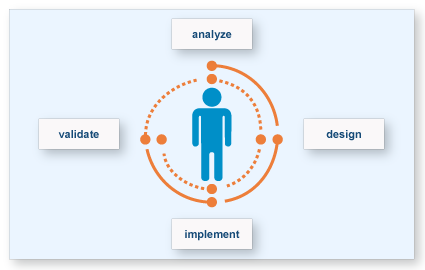
\includegraphics[width=0.7\columnwidth]{user.png}
\caption[Desenvolvimento Centrado no Utilizador] {Desenvolvimento Centrado no Utilizador\protect\footnotemark}
\label{fig:user-center}
\end{figure}

\footnotetext{http://www.medical-safety-design.de/en/medical-safety-design/user-centered-interface-design/}

\begin{itemize}
\item \textbf{Analisar} - Engloba a recolha de requisitos, tendo em conta o contexto de uso e o propósito de desenvolvimento;
\item \textbf{Design} - Projeta possíveis soluções que cumpram o que foi definido na fase anterior;
\item \textbf{Implementar} - Desenvolvimento de protótipos que tornem percetíveis as soluções idealizadas, nos quais os conceitos têm de ser implementados;
\item \textbf{Validar} - Avaliação, por parte de especialistas, da usabilidade e possíveis riscos tendo em conta os requisitos do utilizador final e os conceitos envolvidos.
\end{itemize} 

As etapas acima referidas ocorrem de forma iterativa, existindo uma avaliação de desempenho no final de cada iteração. Inicialmente, na fase de análise são definidos os diversos elementos esperados e analisados em detalhe. Seguem-se as restantes fases, ocorrendo os respetivos testes na fase de validação, que fornece \textit{feedback} em cada iteração. A solução pode ser redefinida numa próxima fase de análise de acordo com os resultados obtidos. 




\section{Fases de Desenvolvimento}

	Enquanto projeto de \textit{software}, é importante uma fase inicial que permita especificar aquilo que se pretende implementar de modo a não divagar. Deste modo será mais fácil que o resultado obtido não fique aquém do que é pretendido.

	Por conseguinte, são definidas as etapas previstas, na realização deste projeto, que levarão à solução final:

	\begin{itemize}
		\item definir as aplicações que são pretendidas como exemplo;
		\item estudar que tipo de controlos serão úteis para as aplicações definidas;
		\item definir a arquitetura do sistema;
		\item escolher as tecnologias usadas para a implementação;
	\end{itemize}  

	Os pontos acima mencionados, funcionarão como guias iniciais antes do desenvolvimento começar, permitindo ter uma ideia do que será necessário ao longo de todo o projeto.
	Torna-se relevante definir que aplicações se pretende desenvolver, tal como os tipos de controlo, pois existem em grande número, não facilitando a especificação de objetivos. Perceber que arquitetura será usada, servirá para ajudar na posterior escolha de tecnologias.
	
	É desejado que sempre que uma aplicação é desenvolvida, a mesma seja testada por utilizadores, facultando uma análise sobre o que pode ser melhorado, não se incorrendo nos mesmo erros na aplicação seguinte.

	Ao longo de todo o processo poderão ocorrer pequenos testes que facilitem o desenvolvimento, evitando grandes alterações na fase final. 


